\documentclass[pdf]{beamer}
\mode<presentation>{}
\usetheme{Dresden}
\usepackage{apalike}
\usepackage{graphicx}
\usepackage{mwe,tikz}\usepackage[percent]{overpic}
%% preamble
\title{Importance of Dispersion for Shoaling Waves}
\author{Jordan Pitt, Stephen Roberts and Christopher Zoppou \\ Australian National University}
\newcommand\solidrule[1][0.25cm]{\rule[0.5ex]{#1}{1pt}}
\newcommand\dashedrule{\mbox{\solidrule[2mm]\hspace{2mm}\solidrule[2mm]}}
\newcommand{\dotrule}[1]{%
	\parbox[]{#1}{\dotfill}}

\setbeamertemplate{itemize item}[triangle]

\begin{document}
%% title frame
\begin{frame}
\titlepage
\end{frame}
%% normal frame
\begin{frame}{Introduction}
	\begin{tabular}{l l l l}
		 { \color[RGB]{59,50,164} \usebeamertemplate{itemize item}{} } &Motivation &:& Tsunamis \\
		 { \color[RGB]{59,50,164} \usebeamertemplate{itemize item}{} } &Model &:& Shallow Water Wave and Serre equations \\
		 { \color[RGB]{59,50,164} \usebeamertemplate{itemize item}{} } &Experiment &:& Comparison of numerical solutions
	\end{tabular}
\end{frame}

\section{Motivation}
\subsection{Tsunamis}
\begin{frame}{Indian ocean tsunami}
		\begin{figure}
			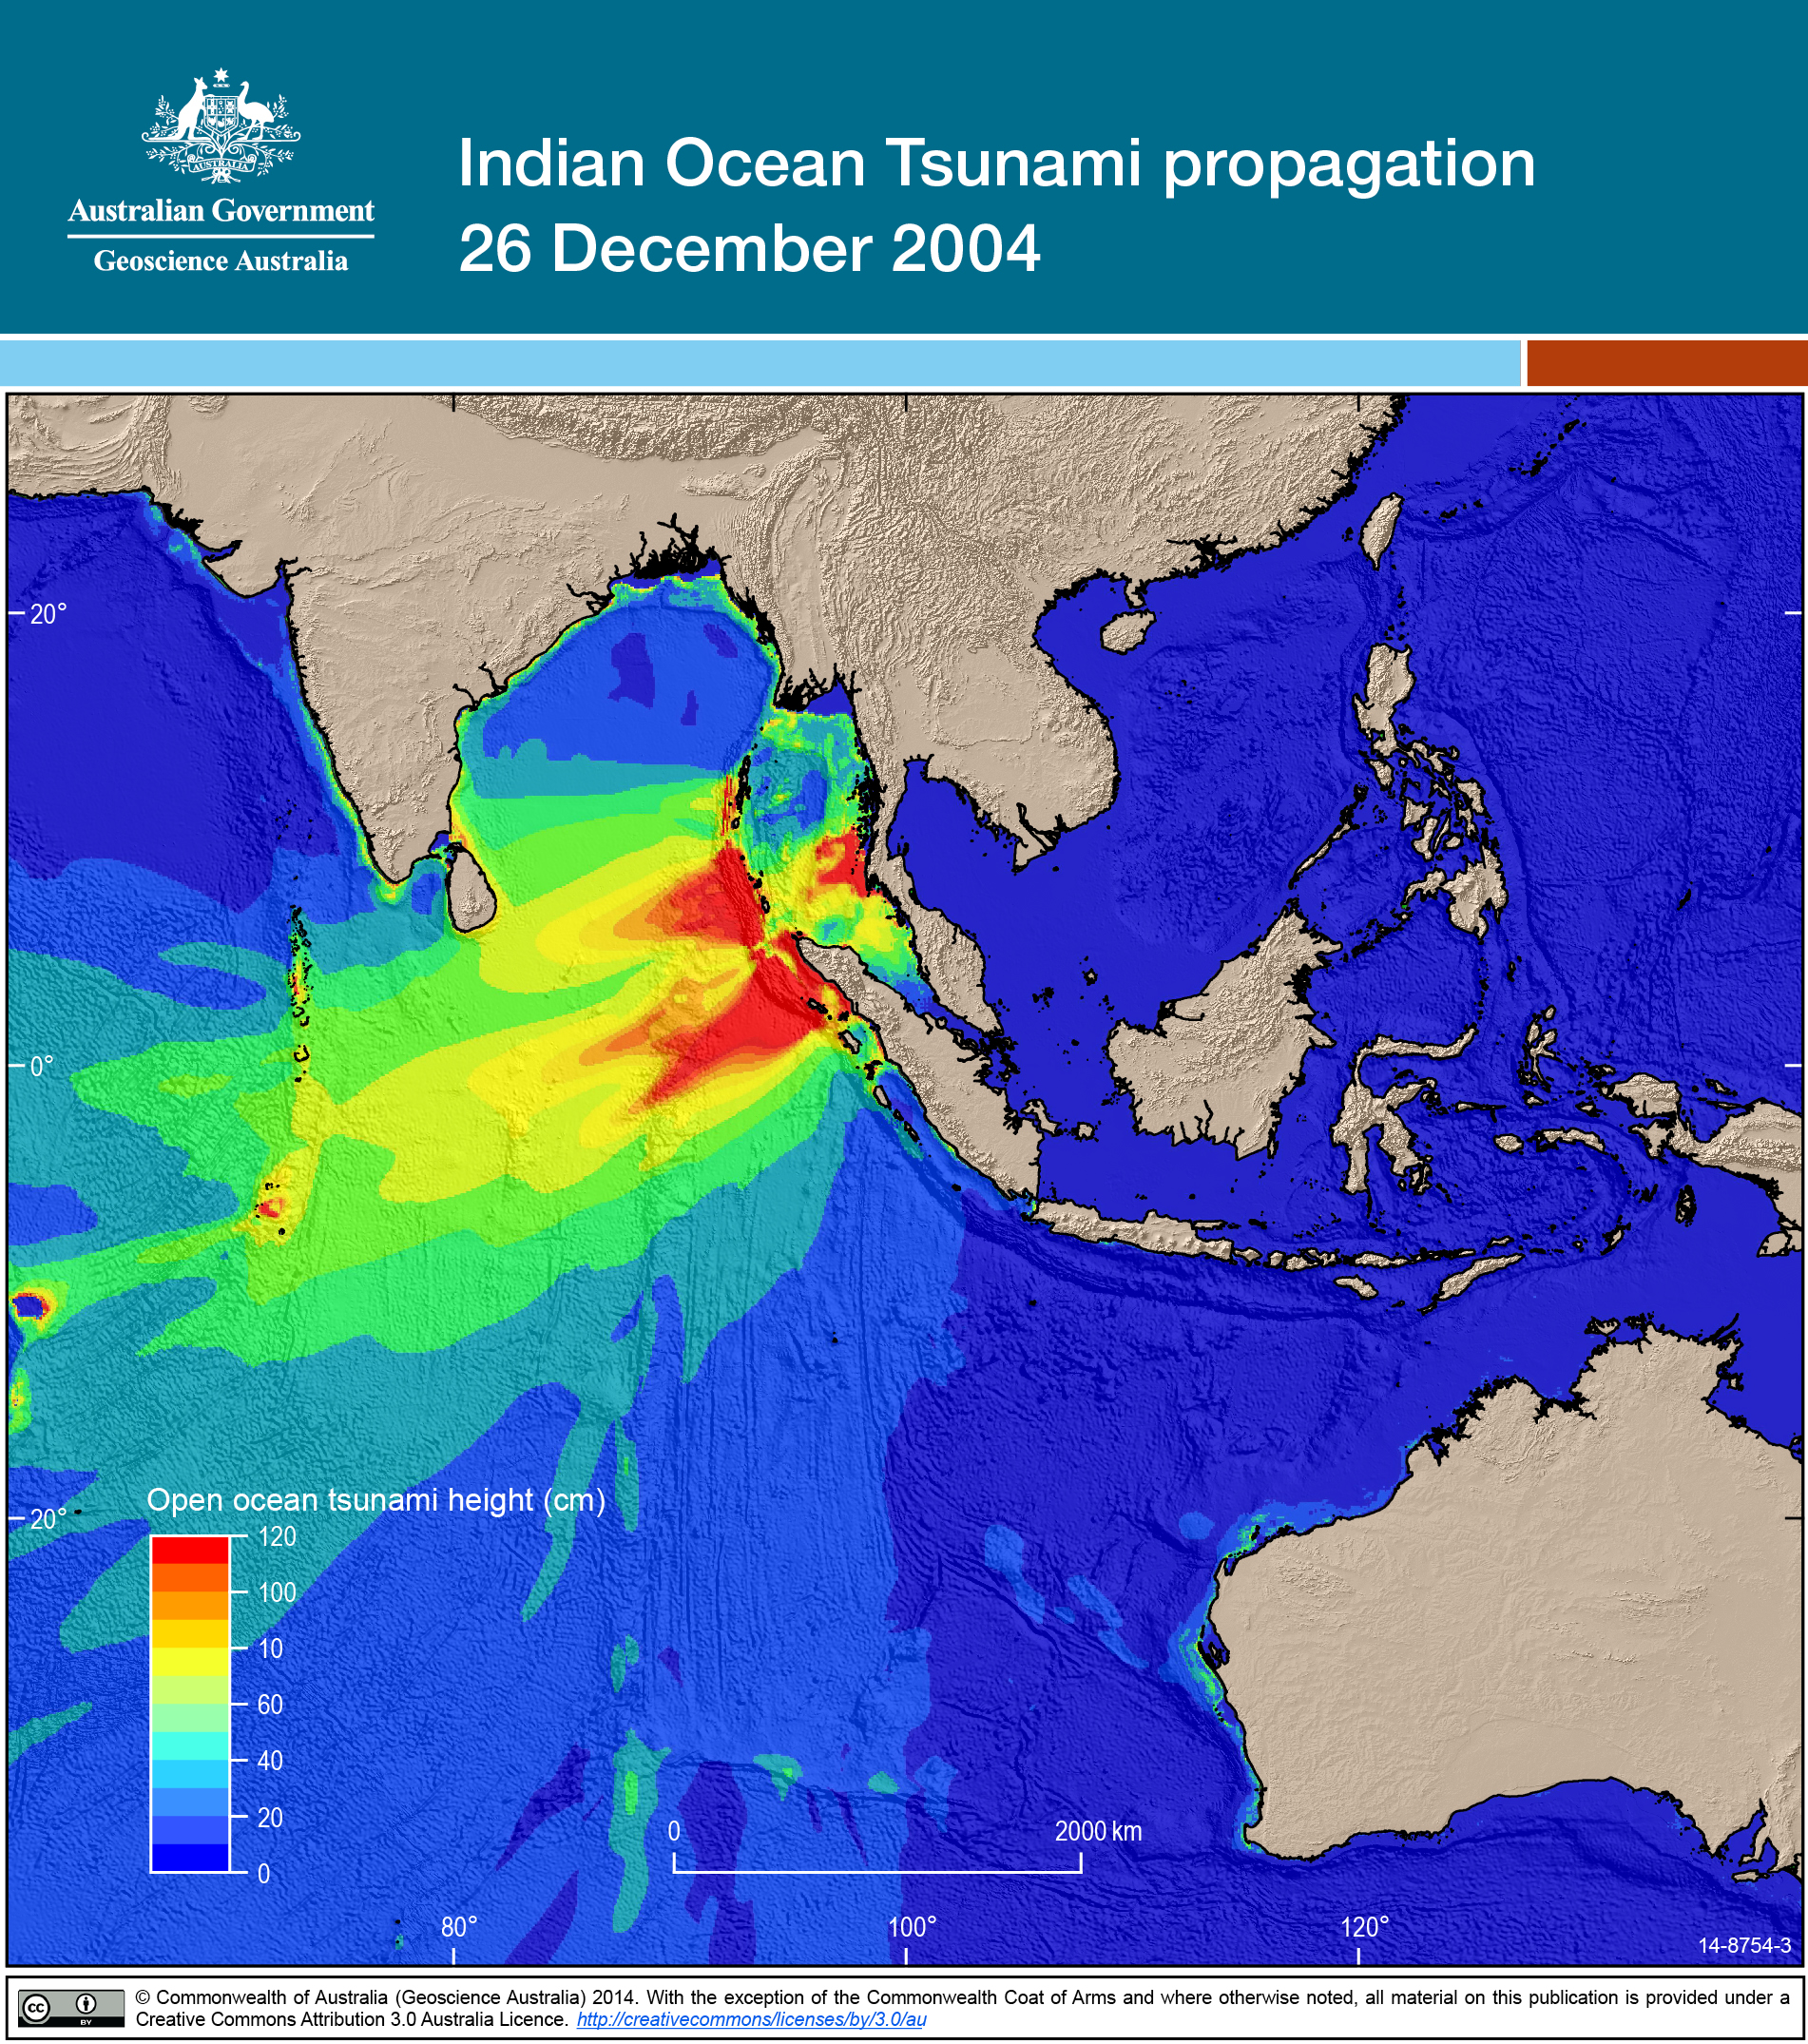
\includegraphics[width=5cm]{./Pics/IOT.jpg}
		\end{figure}
\end{frame}

\begin{frame}{Tsunami diagram}
		\begin{figure}
			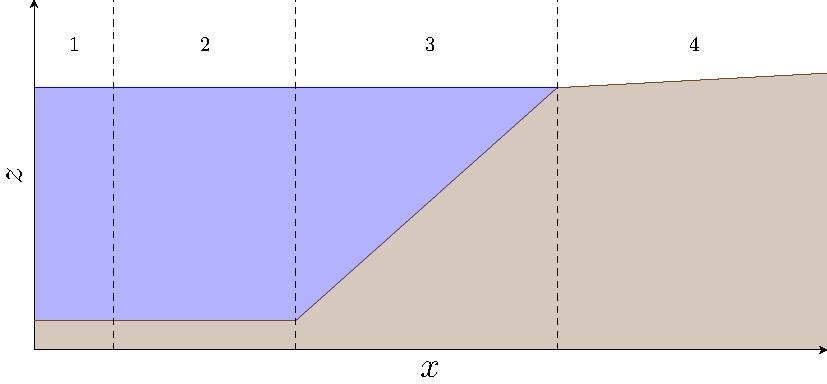
\includegraphics[width=10cm]{./Pics/TsunamiStages.pdf}
		\end{figure}
\end{frame}

\begin{frame}{{\color{red} 1} : Generation}
	\begin{figure}
		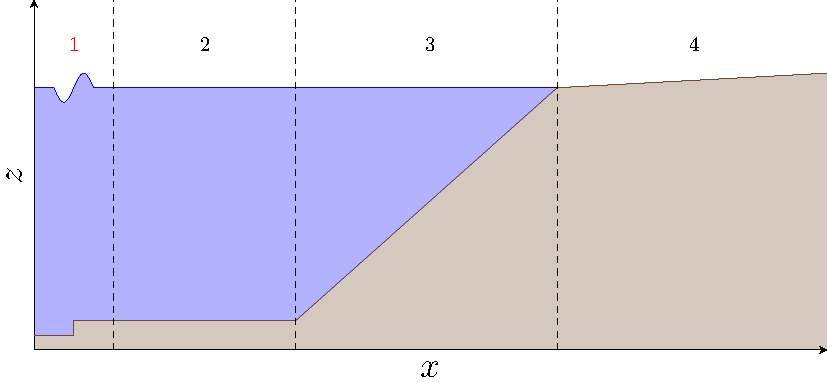
\includegraphics[width=10cm]{./Pics/Tsunami1.pdf}
	\end{figure}
\end{frame}

\begin{frame}{{\color{red} 2} : Propagation far from coast }
	\begin{figure}
		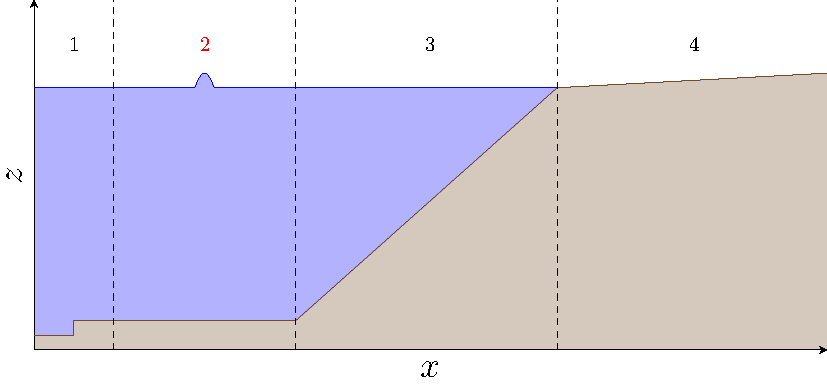
\includegraphics[width=10cm]{./Pics/Tsunami2.pdf}
	\end{figure}
\end{frame}

\begin{frame}{{\color{red} 3} : Propagation near coast }
	\begin{figure}
		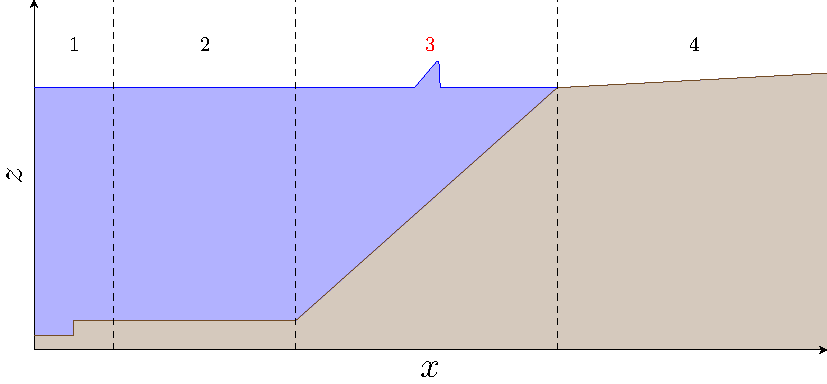
\includegraphics[width=10cm]{./Pics/Tsunami3.pdf}
	\end{figure}
\end{frame}

\begin{frame}{{\color{red} 4} : Inundation }
	\begin{figure}
		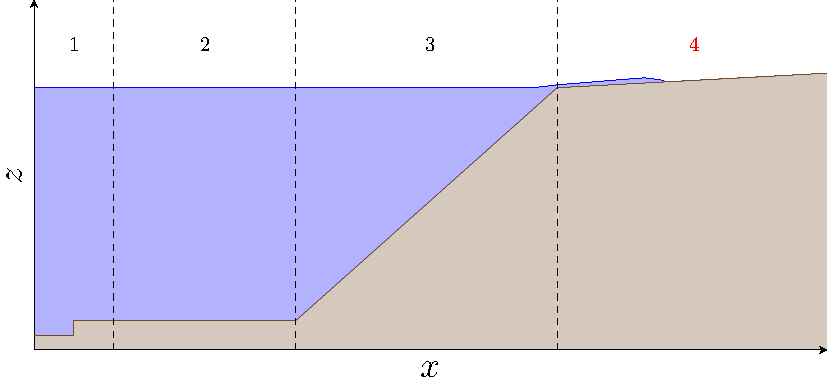
\includegraphics[width=10cm]{./Pics/Tsunami4.pdf}
	\end{figure}
\end{frame}

\section{Model}
\subsection{Depth averaged equations}

\begin{frame}{Depth averaged equations}
		\begin{figure}
			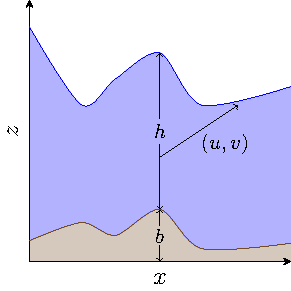
\includegraphics[width=6cm]{./Pics/SWWE.pdf}
		\end{figure}
\end{frame}

\subsection{Shallow water wave equations}
\begin{frame}{Shallow water wave equations}
	\begin{itemize}
		\item Wavelengths ($\lambda$) $>>$ Water depth ($H$) ($\lambda \ge 20 H$)
		\smallskip
		\item Horizontal velocity constant over $z$
		\item Vertical velocity is $0$
		\item Pressure is hydrostatic $p(z) = \rho g(h + b - z)$
	\end{itemize}
\end{frame}

\begin{frame}{Shallow water wave equations}
		Conservation of Mass
		\begin{gather*}
		\dfrac{\partial h}{\partial t} + \dfrac{\partial (uh)}{\partial x} = 0
		\end{gather*}
		Conservation of Momentum
		\begin{gather*}
		\dfrac{\partial (uh)}{\partial t} + \dfrac{\partial}{\partial x} \left ( u^2h + \dfrac{gh^2}{2}\right ) + gh \frac{\partial b}{\partial x} = 0 
		\label{eq:Serre_momentum}
		\end{gather*}
\end{frame}

%phi =\left [ \dfrac{\partial u }{\partial x} \dfrac{\partial u}{\partial x} -u \dfrac{\partial^2 u}{\partial x^2}  - \dfrac{\partial^2 u}{\partial x \partial t}\right ] 

\subsection{Serre equations}
\begin{frame}{Serre equations}
		\begin{itemize}
			\item No restrictions
			\smallskip
			\item Horizontal velocity is constant over $z$
			\item Vertical velocity is linear in $z$
						 $$v'(z) = u\frac{\partial b}{\partial x} - (z - b)\frac{\partial u}{\partial x}$$
		    \item Pressure
		    $$p(z) = {\color{blue} \rho g(h + b - z)} + \rho(h + b - z)  {\color{red} \Psi }  + \frac{\rho}{2}(h+b - z)(h - b + z) {\color{red} \Phi } $$
			\end{itemize}
		\[ {\color{red} \Psi }  = \dfrac{\partial b}{\partial x}\left(\dfrac{\partial u}{\partial t} + u\dfrac{\partial u}{\partial x} \right)  + u^2\dfrac{\partial b}{\partial x} \;, \; 
		{\color{red} \Phi }  = \dfrac{\partial u }{\partial x} \dfrac{\partial u}{\partial x} -u \dfrac{\partial^2 u}{\partial x^2}  - \dfrac{\partial^2 u}{\partial x \partial t}  \]
\end{frame}

\begin{frame}{Serre equations}
	
	    Conservation of Mass
	    \[
		\dfrac{\partial h}{\partial t} + \dfrac{\partial (uh)}{\partial x} = 0
		\]

		Conservation of Momentum
		\begin{multline*}
				{\color{blue} \dfrac{\partial (uh)}{\partial t} + \dfrac{\partial}{\partial x} \left ( u^2h + \dfrac{gh^2}{2}\right ) + gh \frac{\partial b}{\partial x}}  \\+ \dfrac{\partial}{\partial x} \left ( \dfrac{h^2}{2}{\color{red} \Psi} + \dfrac{h^3}{3}{\color{red} \Phi }   \right ) + \dfrac{\partial b}{\partial x} \left (  h{\color{red} \Psi} + \dfrac{h^2}{2}{\color{red} \Phi }  \right ) = 0
		\end{multline*}
		
		\[ {\color{red} \Psi }  = \dfrac{\partial b}{\partial x}\left(\dfrac{\partial u}{\partial t} + u\dfrac{\partial u}{\partial x} \right)  + u^2\dfrac{\partial b}{\partial x} \;, \; 
		{\color{red} \Phi }  = \dfrac{\partial u }{\partial x} \dfrac{\partial u}{\partial x} -u \dfrac{\partial^2 u}{\partial x^2}  - \dfrac{\partial^2 u}{\partial x \partial t}  \]
\end{frame}

\subsection{Differences}
\begin{frame}{Differences}
	Differences:
	\begin{itemize}
		\item Dispersion
		\item Higher order terms
	\end{itemize}
	Are they important for tsunamis?
\end{frame}


\section{Experiment}
\subsection{Aim}
\begin{frame}{Aim}
	\begin{itemize}
		\item Compare Shallow Water Wave and Serre equations
		\item Highlight different behaviours
		\item Highlight possible impacts these differences could make on current simulations
	\end{itemize}
\end{frame}

\begin{frame}
	Numerical Solvers
	\begin{itemize}
		\item Shallow water wave equations: ANUGA, second-order finite volume method
		\item Serre equations: second-order finite volume method (same technique as ANUGA) and a second-order finite difference method
	\end{itemize}
	\bigskip
	Experiments
	\begin{itemize}
		\item Experimental results of Beji and Battjes (1994)
		\item Artificial example replicating common phenomena
	\end{itemize}
\end{frame}

\subsection{Periodic waves over a submerged bar}
\begin{frame}{Periodic waves over a submerged bar: initial conditions}
		\begin{figure}
			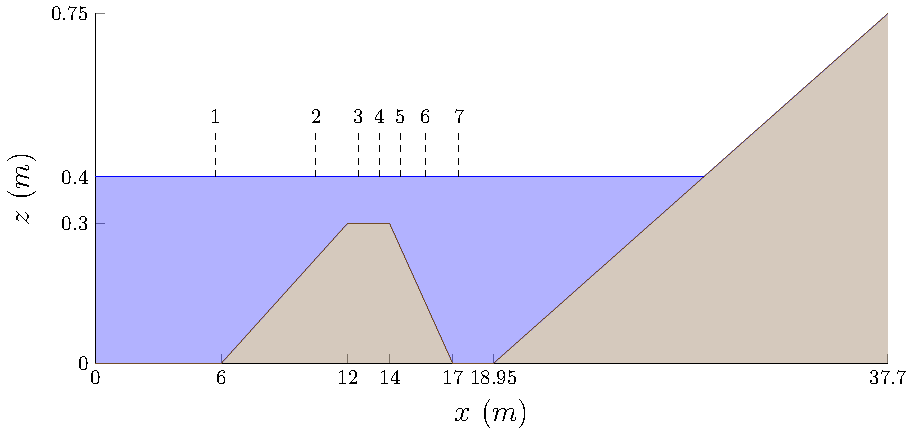
\includegraphics[width=11cm]{./Pics/WT.pdf}
		\end{figure}
\end{frame}

\begin{frame}{Wave gauge 1: boundary condition \space\space	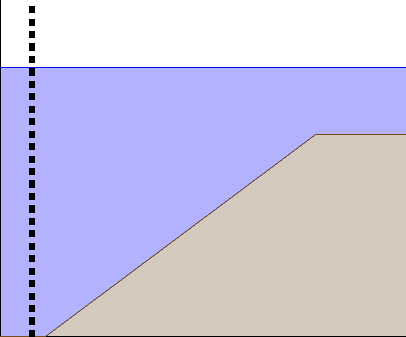
\includegraphics[width=1.2cm]{./Pics/WT1z.pdf} }
    \begin{figure}
    	\centering
    	\begin{minipage}{.5\textwidth}
    		\centering
    		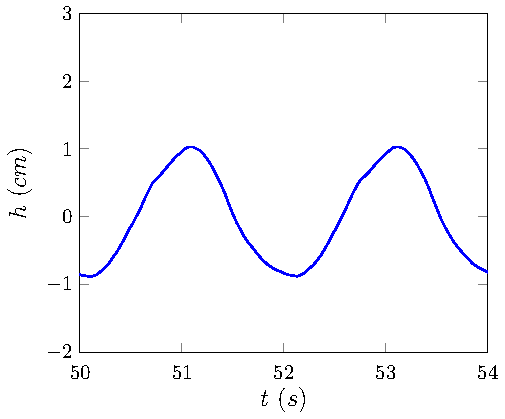
\includegraphics[width=0.9\linewidth]{./Pics/SLWG1.pdf}
    		\caption{Low frequency $\lambda = 3.69m$ and $H = 0.4m$}
    	\end{minipage}%
    	\begin{minipage}{.5\textwidth}
    		\centering
    		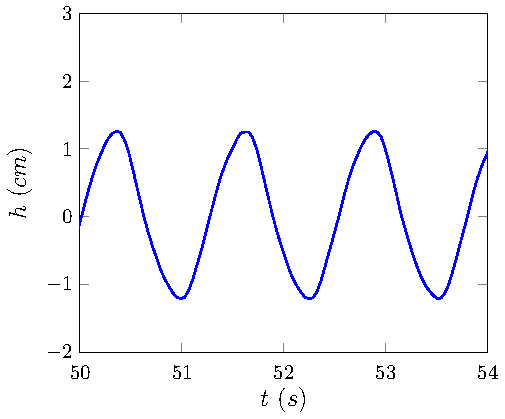
\includegraphics[width=0.9\linewidth]{./Pics/WG1.pdf}
    		\caption{High frequency $\lambda = 2.05m$ and $H = 0.4m$}
    	\end{minipage}
    \end{figure}
\end{frame}

\begin{frame}{Wave gauge 2: experimental result \space\space	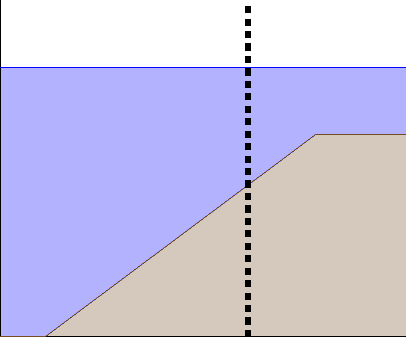
\includegraphics[width=1.2cm]{./Pics/WT2z.pdf}  }
    \begin{figure}
    	\centering
    	\begin{minipage}{.5\textwidth}
    		\centering
    		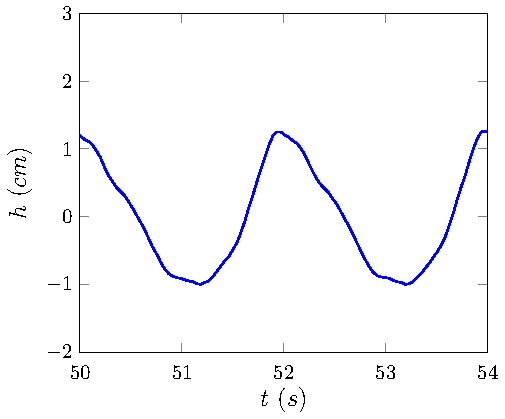
\includegraphics[width=0.9\linewidth]{./Pics/SL/WG2/1e-figure0.pdf}
    		\caption{Low frequency}
    	\end{minipage}%
    	\begin{minipage}{.5\textwidth}
    		\centering
    		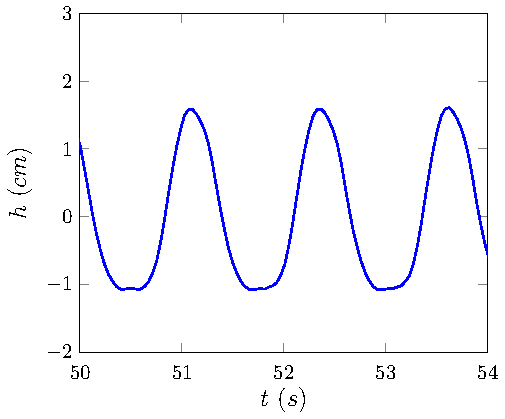
\includegraphics[width=0.9\linewidth]{./Pics/SH/WG2/1e-figure0.pdf}
    		\caption{High frequency}
    	\end{minipage}
    \end{figure}
\end{frame}

\begin{frame}{Wave gauge 2: shallow water wave equation \space\space	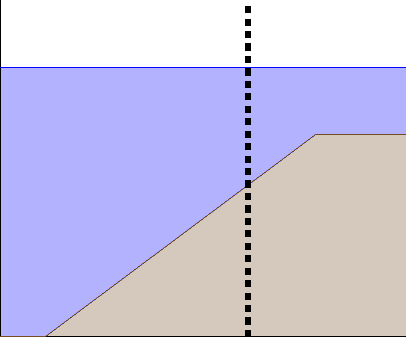
\includegraphics[width=1.2cm]{./Pics/WT2z.pdf}  }
	\begin{figure}
		\centering
		\begin{minipage}{.5\textwidth}
			\centering
			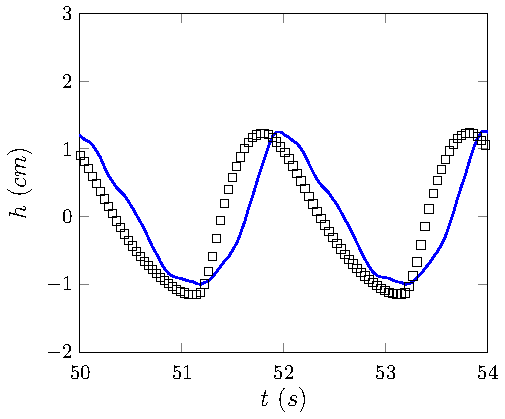
\includegraphics[width=0.9\linewidth]{./Pics/SL/WG2/1SWW-figure0.pdf}
			\caption{Low frequency}
		\end{minipage}%
		\begin{minipage}{.5\textwidth}
			\centering
			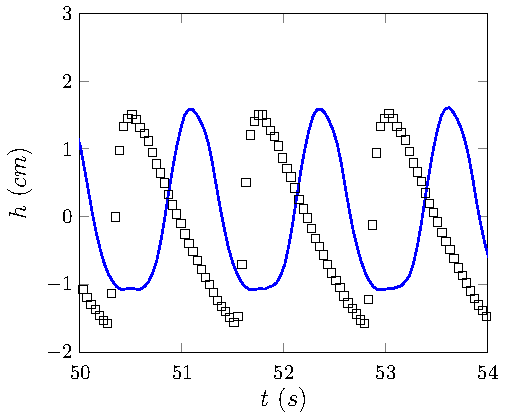
\includegraphics[width=0.9\linewidth]{./Pics/SH/WG2/1SWW-figure0.pdf}
			\caption{High frequency}
		\end{minipage}
	\end{figure}
\end{frame}

\begin{frame}{Wave gauge 2: all results \space\space	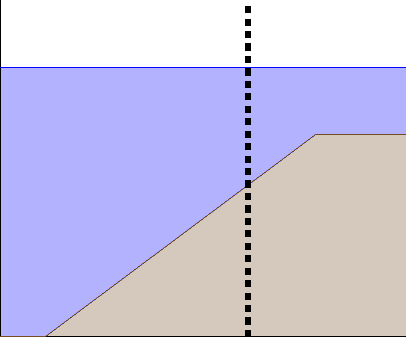
\includegraphics[width=1.2cm]{./Pics/WT2z.pdf}  }
	\begin{figure}
		\centering
		\begin{minipage}{.5\textwidth}
			\centering
			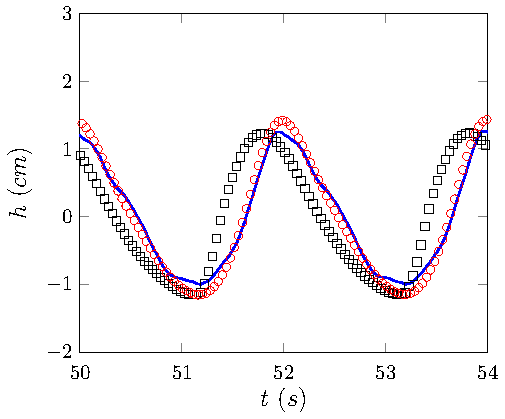
\includegraphics[width=0.9\linewidth]{./Pics/SL/WG2/1-figure0.pdf}
			\caption{Low frequency}
		\end{minipage}%
		\begin{minipage}{.5\textwidth}
			\centering
			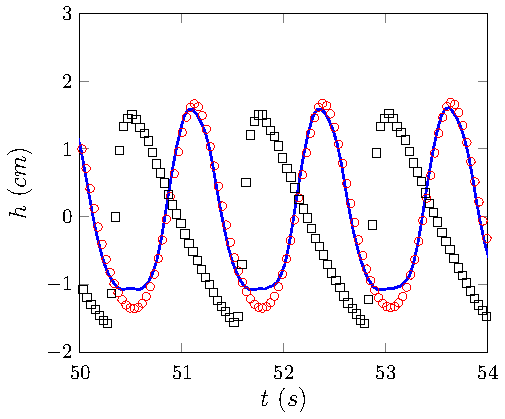
\includegraphics[width=0.9\linewidth]{./Pics/SH/WG2/1-figure0.pdf}
			\caption{High frequency}
		\end{minipage}
	\end{figure}
\end{frame}
\subsection{Periodic waves over a submerged bar}
\begin{frame}{Wave gauge 3: experimental result \space\space	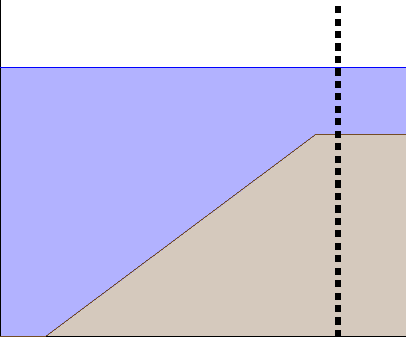
\includegraphics[width=1.2cm]{./Pics/WT3z.pdf}  }
	\begin{figure}
		\centering
		\begin{minipage}{.5\textwidth}
			\centering
			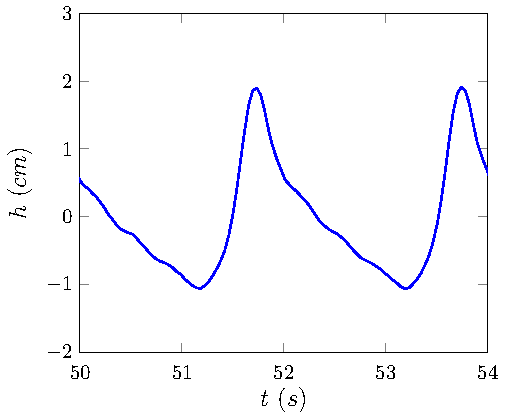
\includegraphics[width=0.9\linewidth]{./Pics/SL/WG3/1e-figure0.pdf}
			\caption{Low frequency}
		\end{minipage}%
		\begin{minipage}{.5\textwidth}
			\centering
			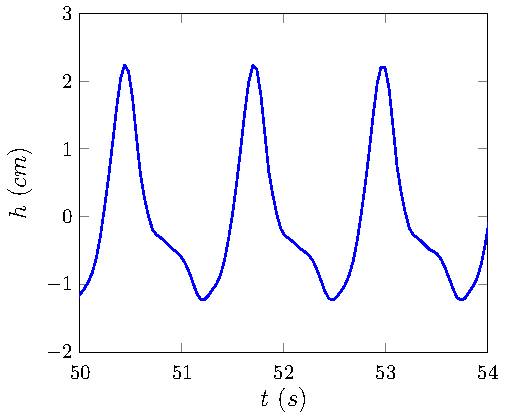
\includegraphics[width=0.9\linewidth]{./Pics/SH/WG3/1e-figure0.pdf}
			\caption{High frequency}
		\end{minipage}
	\end{figure}
\end{frame}

\begin{frame}{Wave gauge 3: shallow water wave equation \space\space	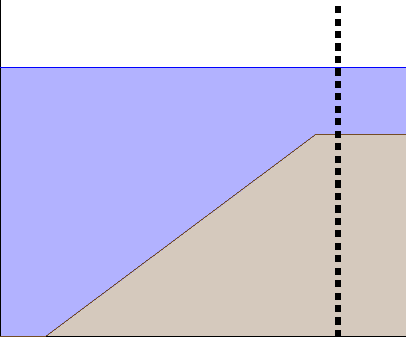
\includegraphics[width=1.2cm]{./Pics/WT3z.pdf}  }
	\begin{figure}
		\centering
		\begin{minipage}{.5\textwidth}
			\centering
			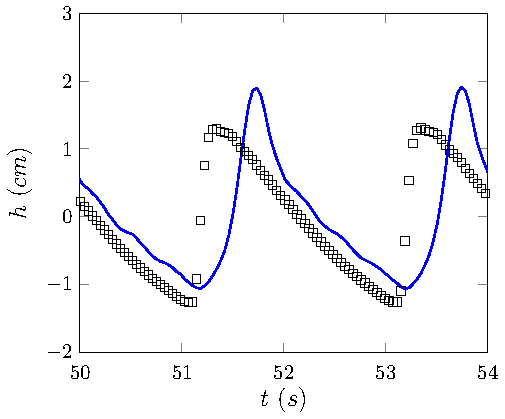
\includegraphics[width=0.9\linewidth]{./Pics/SL/WG3/1SWW-figure0.pdf}
			\caption{Low frequency}
		\end{minipage}%
		\begin{minipage}{.5\textwidth}
			\centering
			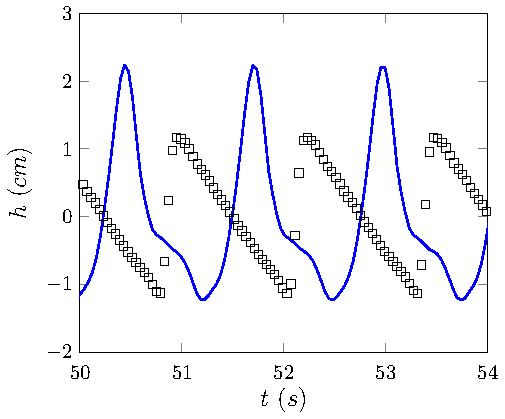
\includegraphics[width=0.9\linewidth]{./Pics/SH/WG3/1SWW-figure0.pdf}
			\caption{High frequency}
		\end{minipage}
	\end{figure}
\end{frame}

\begin{frame}{Wave gauge 3: all results \space\space	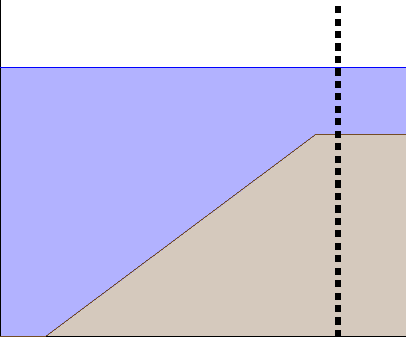
\includegraphics[width=1.2cm]{./Pics/WT3z.pdf}  }
	\begin{figure}
		\centering
		\begin{minipage}{.5\textwidth}
			\centering
			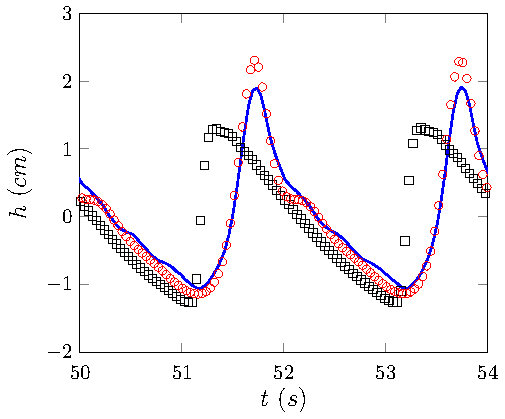
\includegraphics[width=0.9\linewidth]{./Pics/SL/WG3/1-figure0.pdf}
			\caption{Low frequency}
		\end{minipage}%
		\begin{minipage}{.5\textwidth}
			\centering
			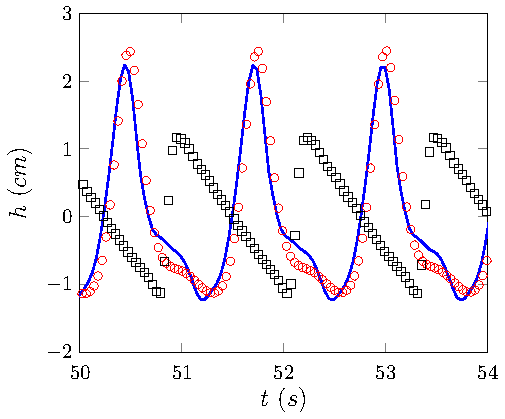
\includegraphics[width=0.9\linewidth]{./Pics/SH/WG3/1-figure0.pdf}
			\caption{High frequency}
		\end{minipage}
	\end{figure}
\end{frame}

\begin{frame}{Wave gauge 4: experimental result \space\space	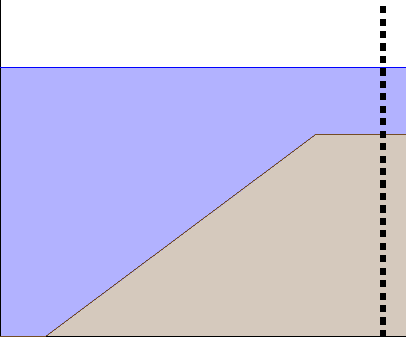
\includegraphics[width=1.2cm]{./Pics/WT4z.pdf}  }
	\begin{figure}
		\centering
		\begin{minipage}{.5\textwidth}
			\centering
			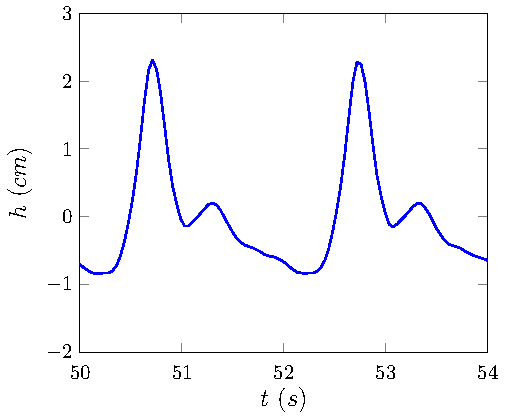
\includegraphics[width=0.9\linewidth]{./Pics/SL/WG4/1e-figure0.pdf}
			\caption{Low frequency}
		\end{minipage}%
		\begin{minipage}{.5\textwidth}
			\centering
			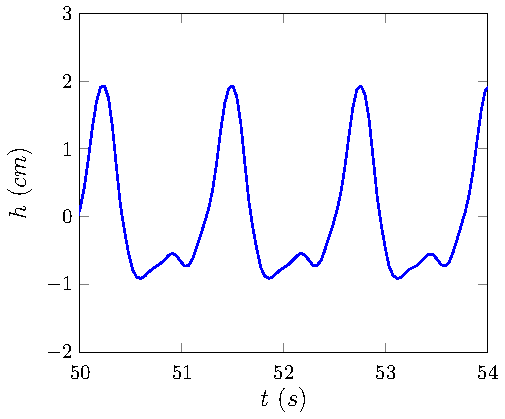
\includegraphics[width=0.9\linewidth]{./Pics/SH/WG4/1e-figure0.pdf}
			\caption{High frequency}
		\end{minipage}
	\end{figure}
\end{frame}

\begin{frame}{Wave gauge 4: shallow water wave equation \space\space	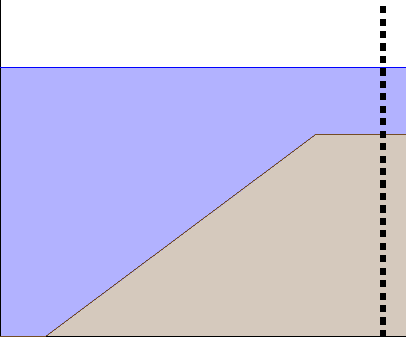
\includegraphics[width=1.2cm]{./Pics/WT4z.pdf}  }
	\begin{figure}
		\centering
		\begin{minipage}{.5\textwidth}
			\centering
			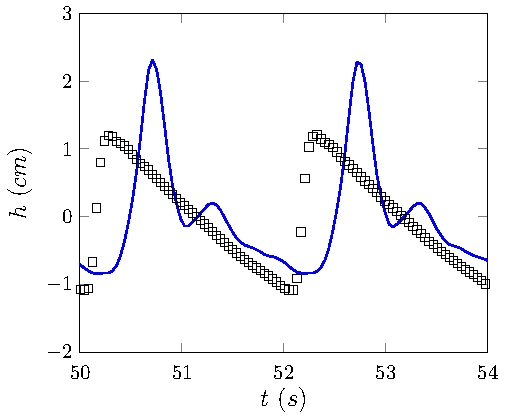
\includegraphics[width=0.9\linewidth]{./Pics/SL/WG4/1SWW-figure0.pdf}
			\caption{Low frequency}
		\end{minipage}%
		\begin{minipage}{.5\textwidth}
			\centering
			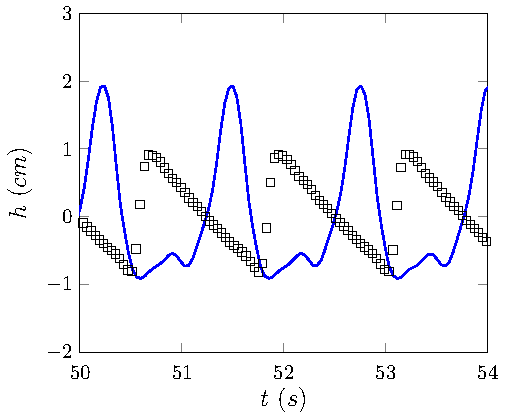
\includegraphics[width=0.9\linewidth]{./Pics/SH/WG4/1SWW-figure0.pdf}
			\caption{High frequency}
		\end{minipage}
	\end{figure}
\end{frame}

\begin{frame}{Wave gauge 4: all results \space\space	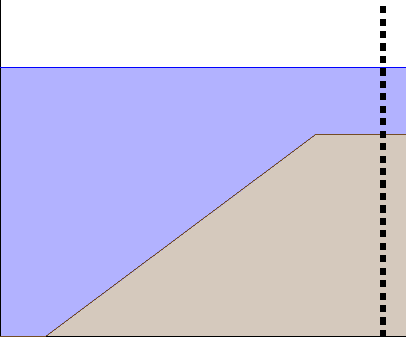
\includegraphics[width=1.2cm]{./Pics/WT4z.pdf}  }
	\begin{figure}
		\centering
		\begin{minipage}{.5\textwidth}
			\centering
			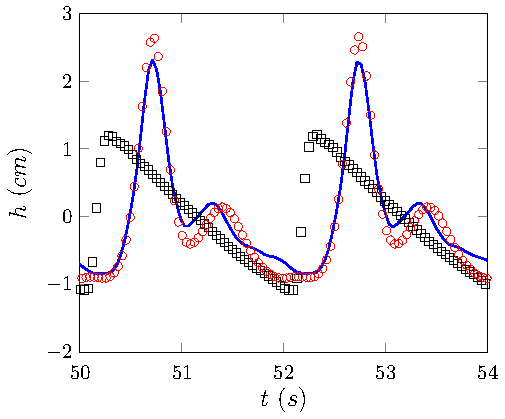
\includegraphics[width=0.9\linewidth]{./Pics/SL/WG4/1-figure0.pdf}
			\caption{Low Frequency}
		\end{minipage}%
		\begin{minipage}{.5\textwidth}
			\centering
			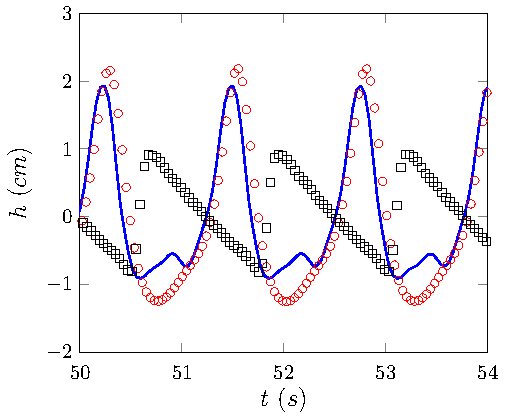
\includegraphics[width=0.9\linewidth]{./Pics/SH/WG4/1-figure0.pdf}
			\caption{High Frequency}
		\end{minipage}
	\end{figure}
\end{frame}

\subsection{Solitary wave over a constant slope}
\begin{frame}{Solitary wave over a constant slope: initial conditions}
			\begin{figure}
				\centering
				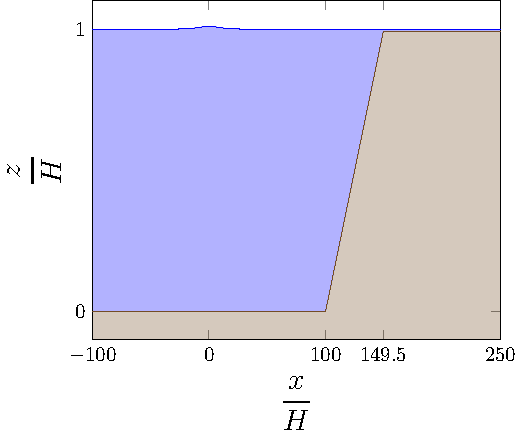
\includegraphics[width=6cm]{./Pics/Diagram/1-figure0.pdf}
			\end{figure}
			\centering
\end{frame}

\begin{frame}{Before slope \space\space 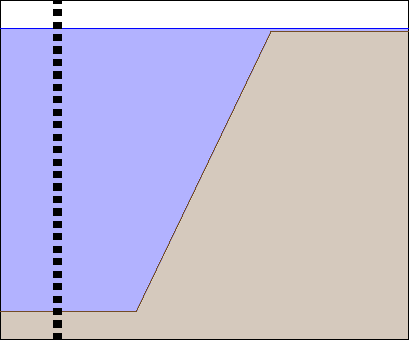
\includegraphics[width=1.2cm]{./Pics/Diagram/1n-figure0.pdf} }
	\begin{figure}
		\centering
		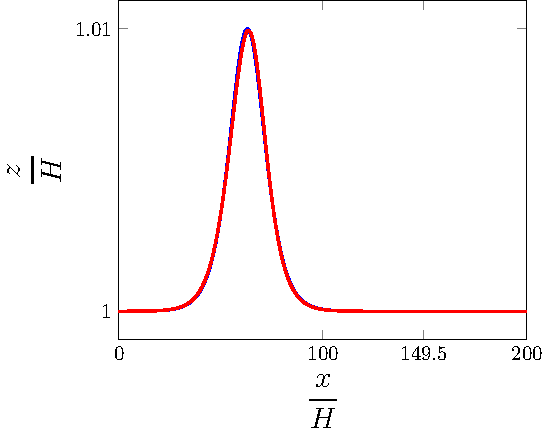
\includegraphics[width=6cm]{./Pics/20s.pdf}
	\end{figure}
\end{frame}

\begin{frame}{Shoaling \space\space 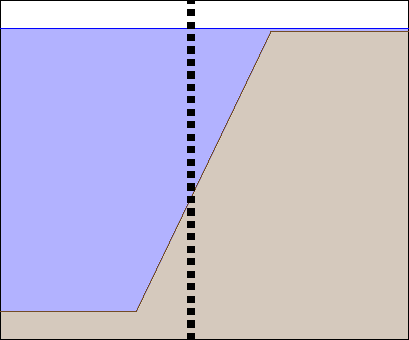
\includegraphics[width=1.2cm]{./Pics/Diagram/1n1-figure0.pdf} }
	\begin{figure}
		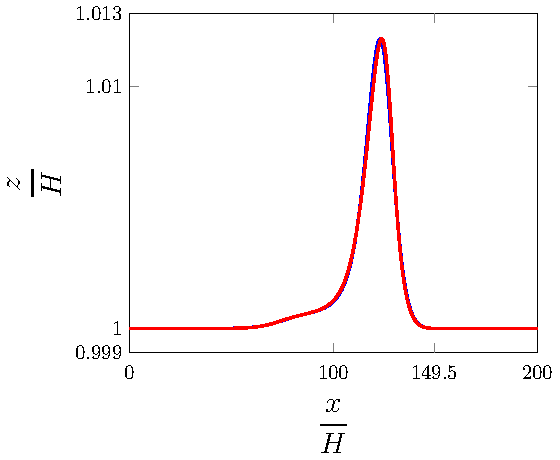
\includegraphics[width=6cm]{./Pics/40s.pdf}
	\end{figure}
\end{frame}

\begin{frame}{Bore formation \space\space 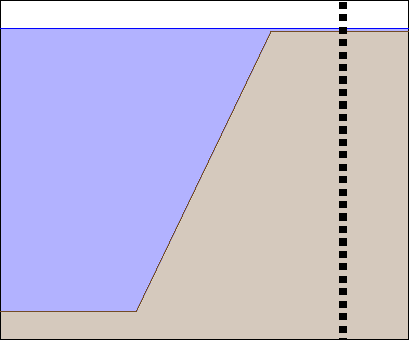
\includegraphics[width=1.2cm]{./Pics/Diagram/1n2-figure0.pdf} }
	\begin{figure}
		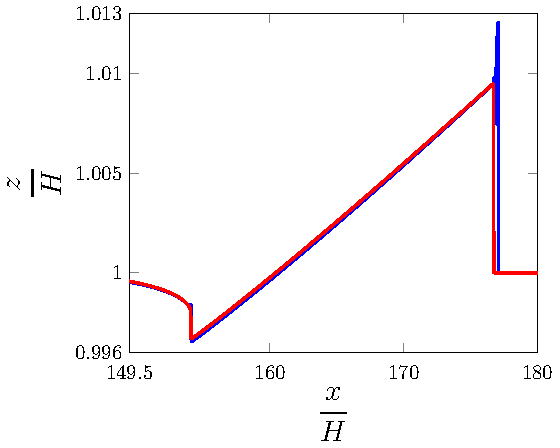
\includegraphics[width=6cm]{./Pics/100s.pdf}
	\end{figure}
\end{frame}

\begin{frame}{Front of bore 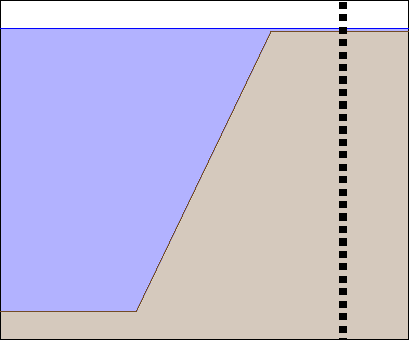
\includegraphics[width=1.2cm]{./Pics/Diagram/1n2-figure0.pdf}}
	\begin{figure}
		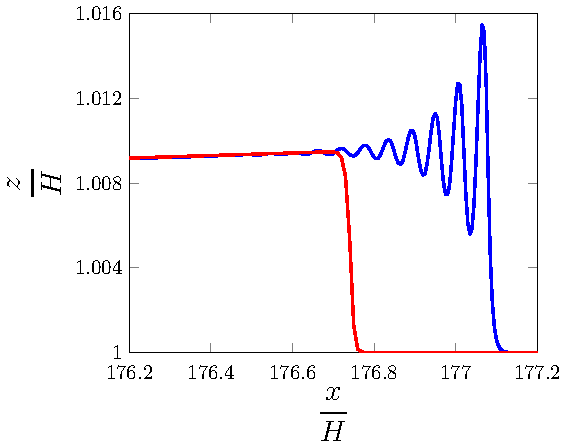
\includegraphics[width=6cm]{./Pics/SerreBore.pdf}
	\end{figure}
\end{frame}

\begin{frame}{Conclusion}
\begin{itemize}
	\item Dispersion plays an important role when wavelengths are not long compared to water depths
	\item Dispersion is not important for shoaling of long wavelength waves
	\item Dispersion is an important effect for waves after shoaling has occurred. 
	\item For shoaled waves our current models may underestimate wave amplitude and predict later arrival times.
\end{itemize}
\end{frame}



\end{document}